% id: 2020-maciel-3-1 | título: Dona Aranha | fonte: listas/2020/Maciel/lista2020maciel3.pdf, p. 1
A Dona Aranha subiu pela parede e fez sua teia no formato de um hexágono regular de lado $l = 45\ cm$ (Figura 1) e fixou as pontas dos fios radiais de raio $r = 10\ \mu m$ de tal maneira que a tensão em cada fio acabou sendo $F_0 = 6,0\ mN$. Assuma que a deformação do fio é elástica e que o módulo de Young é $E = 2,0 \cdot 10^8\ Pa$. Um fio rompe quando a deformação relativa excede $\epsilon_{max} = 0,2$.
\begin{center}
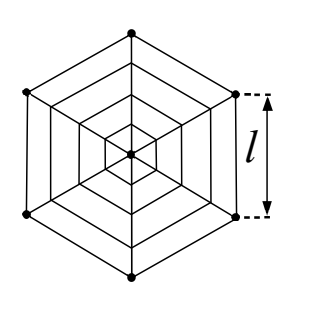
\includegraphics[width=.32\linewidth]{fig/1.png}\\[2pt]
{\small Figura 1: Problema 1}
\end{center}
\begin{enumerate}[label=\textbf{\alph*)}, leftmargin=*]
\item Determine a maior massa $M$ de uma mosca na qual a teia não se rompe ao ser atingida a uma velocidade $v = 2,0\ m/s$. A mosca atinge o centro da teia perpendicularmente ao seu plano.
\item Uma mosca de massa $m = 0,10\ g$ ficou presa no centro da teia. Determine o período $T$ de pequenas oscilações perpendiculares ao plano da teia. Uma vez na teia, uma mosca não consegue mais bater suas asas.
\end{enumerate}
